% % % % % % % % % % % % % % % % % % % % % % % % % % % % % % % % 
% BSc Physics Dissertation
% % % % % % % % % % % % % % % % % % % % % % % % % % % % % % % %
\documentclass[twoside, fontsize=12pt,
     bibliography=totoc, % Include bibliography in contents
     listof=totoc, % Include lists of figures and tables in contents
     index=totoc, % Include index in contents
     onehalfspacing %  or doublespacing
    %,openright
]{_MScDiss2017_cls}

%\usepackage{txfonts,epsfig}
\usepackage[labelfont=footnotesize,textfont=footnotesize]{caption}   
\usepackage{_twoopt}
\usepackage{url}
\usepackage[colorlinks,citecolor=blue,linkcolor=blue,urlcolor=blue,hyperfootnotes=false,linktocpage,breaklinks=true]{hyperref}
%\usepackage{breakurl}
\usepackage[]{_MScDiss_sty}
%\usepackage{chngcntr}
%\counterwithout{footnote}{chapter}

%% these macros turn citations into ADS clickers in dvi, pdf, html output
%% (EDP Sciences improved them in December 2012 to work also with pdflatex)
\bibpunct{(}{)}{;}{a}{}{,}    %% natbib cite format used by A&A and ApJ
\makeatletter
 \newcommandtwoopt{\citeads}[3][][]{\href{http://adsabs.harvard.edu/abs/#3}%
   {\def\hyper@linkstart##1##2{}%
    \let\hyper@linkend\@empty\citealp[#1][#2]{#3}}}    %% Rutten, 2000
 \newcommandtwoopt{\citepads}[3][][]{\href{http://adsabs.harvard.edu/abs/#3}%
   {\def\hyper@linkstart##1##2{}%
    \let\hyper@linkend\@empty\citep[#1][#2]{#3}}}      %% (Rutten 2000)
 \newcommandtwoopt{\citetads}[3][][]{\href{http://adsabs.harvard.edu/abs/#3}%
   {\def\hyper@linkstart##1##2{}%
    \let\hyper@linkend\@empty\citet[#1][#2]{#3}}}      %% Rutten (2000)
 \newcommandtwoopt{\citeyearads}[3][][]%
   {\href{http://adsabs.harvard.edu/abs/#3}%
   {\def\hyper@linkstart##1##2{}%
    \let\hyper@linkend\@empty\citeyear[#1][#2]{#3}}}   %% 2000
\makeatother

\declaration{I hereby certify that this Dissertation, has been written by me at the School of Physics and Astronomy, Queen Mary University of London, that all material in this dissertation which is not my own work has been properly acknowledged, and  that it has not been submitted in any previous application for a higher degree.} 

%--Put your information between here----%
\title{The Effects of Energy Densities on the CMB Power Spectrum}
\author{Daniil Dolgich (150066826)}
\supervisor{Prof. Teppei Katori}
\date{\today}
%\date{July 2019} 
\acknowledgements{I  thank whoever I want here - or I can instead comment it out.}
\newpage % to ensure page 1 starts on front of a page rather than back
%%---and here------%

\begin{document}
\pagenumbering{roman}
\setcounter{tocdepth}{5}

\maketitle
\abstract{We studied the Cosmic Microwave Background radiation (CMB) in order to better understand the lesser studied portions of the CMB Power Spectrum. To facilitate this, I created my own CMB simulator using Python, and used it to demonstrate the effects that different values for Baryonic matter, Dark Matter, and Neutrino energy densities have on the CMB power spectrum.}
\tableofcontents % generates Table of Contents
\listoffigures % generates List of figures
\listoftables % generates List of Tables
Introduction: general overview of what CMB is; what I mean by energy densities; current understanding of CMB (composition etc, observed values); the simulation was created as a way to fit the data, and to find the composition.


Methodology: literally everythind I did to get my simulation running


Results: remarks about the simulations and how the graph changes with varying values of each energy density.


Conclusion: expansion of abstract plus summary of results

\newpage% to flush out last roman numeral
\cleardoublepage
\pagenumbering{arabic}% Set arabic page numbers now that dissertation proper is starting.

% rather than having a very long file you can Input files for each chapter/section here using 
% \input{relative-path-to-file} or just put the files in the same directory as this file.

%Chapter
\chapter{Introduction}
The Cosmic Microwave Background radiation (CMB) is electromagnetic radiation (EM) from the time of the Big Bang. Over the course of around 13 billion years, the CMB has been red-shifted to longer wavelengths due to the persisting expansion of the universe. As such, it has cooled dramatically from its initial state about 300,000 years after the Big Bang. The exact nature of the origins of the CMB and the Big Bang theory are beyond the scope of this project; however, the important part of this is that the CMB is about 2.7 Kelvin above absolute zero.

\paragraph{}

At cosmological scales, about 100 giga parsecs (Gpc), the universe may be taken to be homogeneous and isotropic. In other words, the universe is the same in all locations, and in all directions. The CMB is therefore also considered to be both of these things when looking at such immense scales. However, this is not quite the case for the CMB.

\paragraph{}

One can see in the image of the CMB taken by the Planck satellite that it's quite the opposite in fact. There are many zones of differing temperatures. The CMB is not wholly isotropic and this image shows that very clearly. These fluctuations are incredibly small, within the order of micro-Kelvin, and are collectively known as anisotropy.

\paragraph{}

The way to describe the CMB anisotropy is with spherical harmonics. As such, the CMB power spectrum is actually an angular power spectrum. Under the model of Inflation, these temperature fluctuations are Gaussian, and the variance is given by C\textsubscript{l}. l in this instance is the multipole moment. Different values of l represent a given angle in the sky, and can be thought of as angular frequency for the temperature fluctuations, with higher values of l corresponding to smaller angles.

\paragraph{}

We can see how the plots of the multipole moment against the temperature fluctuations in micro-Kelvin\textsuperscript{2} results in the CMB power spectrum. The three characteristic peaks correspond to the curvature of the universe, the baryon density, and the cold dark matter density, though the exact reasons why are beyond the scope of this research.

\paragraph{}

There are three commonly considered energy densities used to construct the CMB power spectrum: Omega(b)which denotes normal baryonic matter, Omega(c) denotes cold dark matter, and Omega(lambda) denotes dark energy. This however neglects another energy density value, specifically, Omega(nu), the energy density of neutrinos. 

\paragraph{}

With this in mind, I decided to create my own CMB simulator to see exactly how different values for these energy densities affects the power spectrum, and how the overall composition of the universe would change.

\chapter{Methodology}

\section{Preliminary research}
Before I could begin, I had to first familiarise myself with the precise meanings of each element of the CMB power spectrum and how anisotropy was the underlying aspect.

\paragraph{}

I found online, two simulators of the CMB, one simplistic and the other incredibly in-depth. The simplistic one was similar to what I had planned to make myself: a simulator that allows changing of variables and instantly outputs the new graph. The second simulator did not have this feature but had a large selection of variables to tweak.

\paragraph{}

The second simulator, upon completion of the simulation, would also provide a data file in which were contained the multipole moment values ranging from 2 to 2200, as well as the temperature fluctuations for the different versions of the CMB spectrums. The one I was concerned with was the temperature angular power spectrum (TT). I used this file as the input for all the base variables in my simulator. I also looked at the values presented  for the temperature-polarisation cross-power spectrum (TE) and the polarised spectrum (EE), and decided to also simulate these graphs for the purposes of comparison; to see whether they get affected the same way as my baseline TT graph. There was no intent to delve deeper into the effects of the polarisation.

\section{Making the simulator}




\label{sec:template}


\begin{figure}[hbtp]
  \begin{center}
  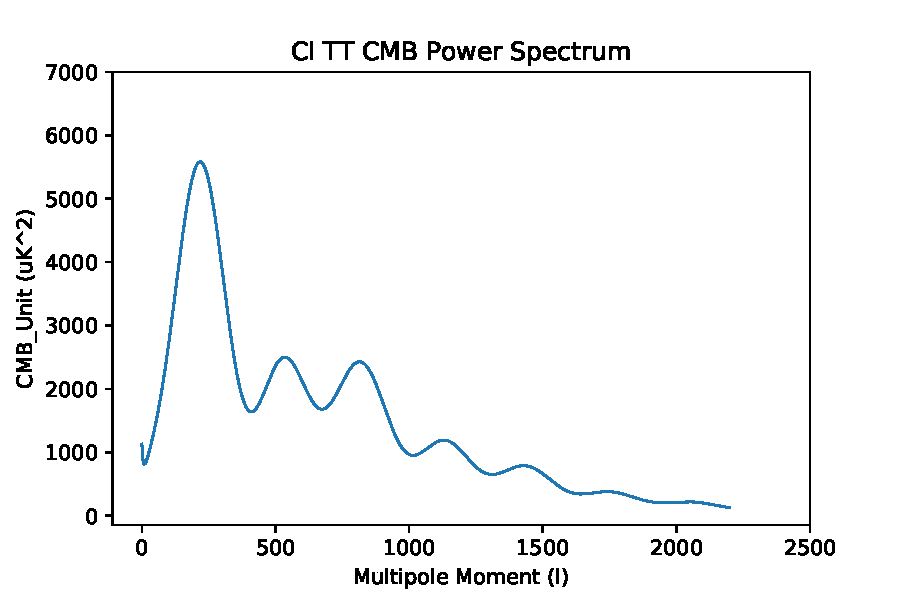
\includegraphics[width=80mm]{Cl-TT-vs-l.pdf}
  \caption{Scalar Non-lensed CMB Power Spectrum TT} 
  \label{fig:test}
  \end{center}
\end{figure}

%%BIBLIOGRAPHY SECTION
\begin{singlespace}% Start single space for bibliography
\bibliographystyle{_abbrvnat_jpe}    
\bibliography{Surname,bib-aanda,bib-apj,bib-astronj,bib-mnras,bib-stateqm,bib-various} %makes BIBLIOGRAPHY from the listed bib files  
\end{singlespace}

\end{document}
